\begin{frame}{Evaluation}

  Benchmark:
  \begin{itemize}
  \item \textbf{Numerical Differentiation}
  \item \textbf{Black Scholes}
  \item \textbf{Reverse Time Migration}
  \item \textbf{Bitonic Sorting Network}
  \item \textbf{Ad Prediction}
  \end{itemize}
\end{frame}

\begin{frame}{Evaluation: Reverse Time Migration}
  \begin{itemize}
  \item seismic imaging application for oil and gas exploration
  \item 3 dataflow kernels
    \begin{itemize}
    \item RTM -- compute intensive, multiple configurations
    \item CmdWrite -- memory write command generator
    \item CmdRead -- memory read command generator
    \end{itemize}
  \item computationally demanding
  \item   use run-time reconfiguration to improve performance and efficiency
  \end{itemize}
\end{frame}

\begin{frame}{Evaluation: RTM Design Space Exploration}
\begin{figure}[!h]
  \centering
  \hspace{-2cm}
  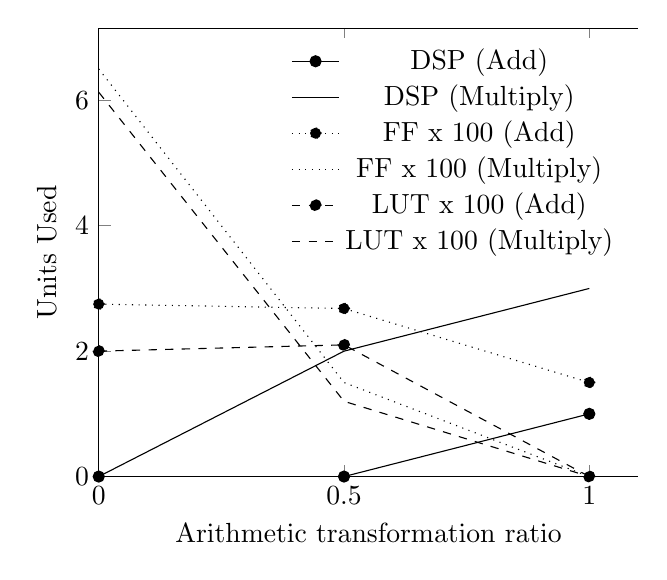
\begin{tikzpicture}
    \selectcolormodel{gray}
    \begin{axis}[
      xmin=0,
      ymin=0,
      axis y line*=left,
      xlabel=Arithmetic transformation ratio,
      ylabel=Units Used,
      xtick={0, 0.5, 1},
      legend columns=1,
      legend entries={
        DSP (Add),
        DSP (Multiply),
        FF x 100 (Add),
        FF x 100 (Multiply),
        LUT x 100 (Add),
        LUT x 100 (Multiply),
      },
      legend style={
        draw=none
      }
      ]
      \addplot[mark=*] coordinates {
        (0, 0)
        (0.5, 0)
        (1, 1)
      };
      \addplot[] coordinates {
        (0, 0)
        (0.5, 2)
        (1, 3)
      };
      \addplot[mark=*, dotted] coordinates {
        (0, 2.75)
        (0.5, 2.68)
        (1, 1.50)
      };
     \addplot[dotted] coordinates {
        (0, 6.5)
        (0.5, 1.5)
        (1, 0)
      };
      \addplot[mark=*, dashed] coordinates {
        (0, 2)
        (0.5, 2.1)
        (1, 0)
      };
      \addplot[dashed] coordinates {
        (0, 6.13)
        (0.5, 1.2)
        (1, 0)
      };
    \end{axis}
  \end{tikzpicture}
\end{figure}
\end{frame}

\begin{frame}{Evaluation: RTM Word Length Exploration}
\vspace{-0.5cm}
\begin{figure}
  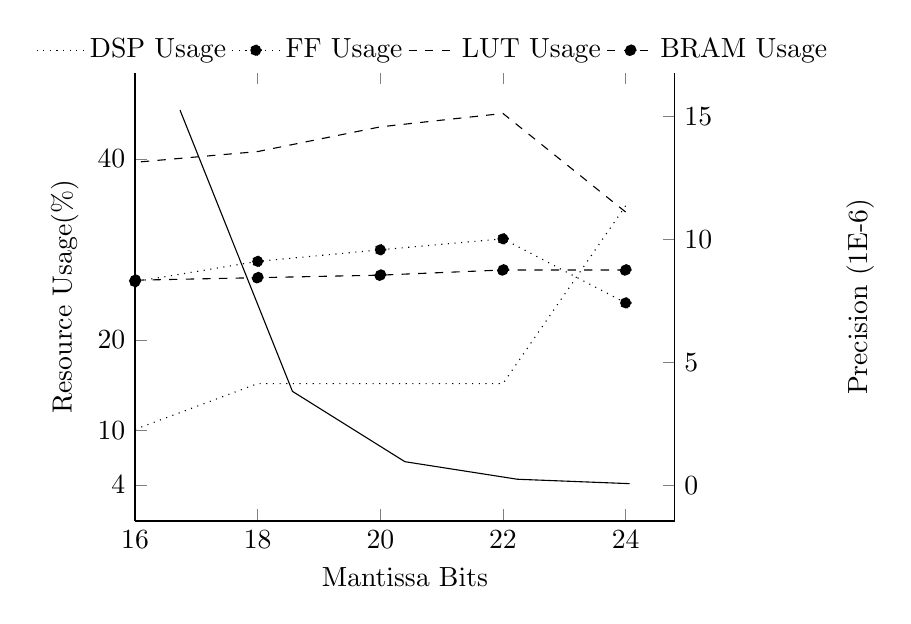
\begin{tikzpicture}
    \selectcolormodel{gray}
    \begin{axis}[
      xmin=16,
      ymin=0,
      axis y line*=left,
      xlabel=Mantissa Bits,
      ylabel=Resource Usage(\%),
      xtick={16,18,20,22,24},
      ytick={4, 10, 20, 40, 50, 70, 80, 100},
      legend columns=4,
      legend entries={
        DSP Usage,
        FF Usage,
        LUT Usage,
        BRAM Usage},
      legend style={
        draw=none,
        at={(-0.2,1.05)},
        anchor=west
      }
      ]
      \addplot[dotted] coordinates {
        (24, 34.82)
        (22, 15.18)
        (20, 15.18)
        (18, 15.18)
        (16, 10.12)
      };
      \addplot[mark=*, dotted] coordinates {
        (24, 24.09)
        (22, 31.17)
        (20, 29.96)
        (18, 28.68)
        (16, 26.44)
      };
      \addplot[mark=none, dashed] coordinates {
        (24, 34.13)
        (22, 45.02)
        (20, 43.54)
        (18, 40.81)
        (16, 39.62)
      };
      \addplot[mark=*, dashed] coordinates {
        (24, 27.73)
        (22, 27.73)
        (20, 27.16)
        (18, 26.88)
        (16, 26.60)
      };
    \end{axis}
    \begin{axis}[
      ylabel=Precision (1E-6),
      axis y line*=right,
      axis x line=none,
      ylabel style={at={(1.3,0.5)}}
      ]
      \addplot[mark=none] coordinates {
        (16, 15.2585)
        (18, 3.8146)
        (20, 0.9536)
        (22, 0.2394)
        (24, 0.0596)
      };
    \end{axis}
  \end{tikzpicture}
\end{figure}
\end{frame}

\begin{frame}{Evaluation: RTM Parallelism}
\begin{figure}[!h]
  \centering
  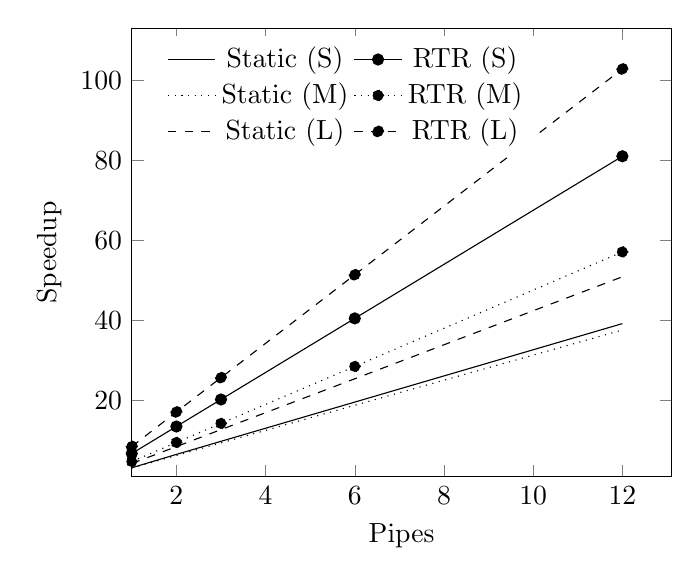
\begin{tikzpicture}
    \begin{axis}[
      xmin=1,
      ymin=1,
      xlabel=Pipes,
      ylabel=Speedup,
%      xtick={1,2,3,6,12},
%      ytick={4, 10, 20, 40, 50, 70, 80, 100},
      legend columns=2,
      legend entries={
        Static (S),
        RTR (S),
        Static (M),
        RTR (M),
        Static (L),
        RTR (L)},
      legend style={
        draw=none,
        at={(0.05,0.85) },
        anchor=west
      }
      ]
      \addplot[mark=none] coordinates {
        (1, 3.2)
        (2, 6.53)
        (3, 9.8)
        (6, 19.6)
        (12, 39.2)
      };
      \addplot[mark=*] coordinates {
        (1, 6.75)
        (2, 13.5)
        (3, 20.25)
        (6, 40.5)
        (12, 81)
      };
      \addplot[dotted] coordinates {
        (1, 3.13)
        (2, 6.26)
        (3, 9.4)
        (6, 18.8)
        (12, 37.6)
      };
      \addplot[mark=*, dotted] coordinates {
        (1, 4.75)
        (2, 9.51)
        (3, 14.27)
        (6, 28.5)
        (12, 57.1)
      };
      \addplot[mark=none, dashed] coordinates {
        (1, 4.25)
        (2, 8.48)
        (3, 12.725)
        (6, 25.42)
        (12, 50.9)
      };
      \addplot[mark=*, dashed] coordinates {
        (1, 8.5)
        (2, 17.13)
        (3, 25.7)
        (6, 51.4)
        (12, 102.8)
      };
    \end{axis}
  \end{tikzpicture}
\end{figure}



\end{frame}


\begin{frame}{Evaluation: Benchmark}
  Comparing manual MaxCompiler designs to FAST designs:
  \begin{table}
    \renewcommand{\arraystretch}{1.2}
    \begin{tabular}{l|p{1cm}|p{1cm}|c|p{2cm}}
      \textbf{Kernel} & \textbf{LOC} & \textbf{API Calls} & \textbf{Performance}              & \textbf{Resource}
                                                                                                                                         \\
      \hline\hline
      CmdRead         & 1.76               & 4.33                     & \multirow{2}{*}{$ > 75\%$}        & \multirow{6}{3cm}{$\approx 100\%$} \\
      CmdWrite        & 1.45               & 4.13                     &                                   &                              \\
      \cline{1-4}
      RTM             & 1.17               & 10                       & \multirow{5}{*}{$ \approx 100\%$} &                              \\
      SGSmooth        & 1.85               & 14                       &                                   &                              \\
      SGDifff         & 1.75               & 14                       &                                   &                              \\
      Black-Scholes   & 2.51               & 5.5                      &                                   &                              \\
      \cline{5-5}
      Add Prediction  & 1.67               & 16                       &                                   &    $ \approx 123 \% $                          \\
    \end{tabular}
  \end{table}

\end{frame}